\subsection{DIRC signal}

\begin{figure}[!h]
\centering
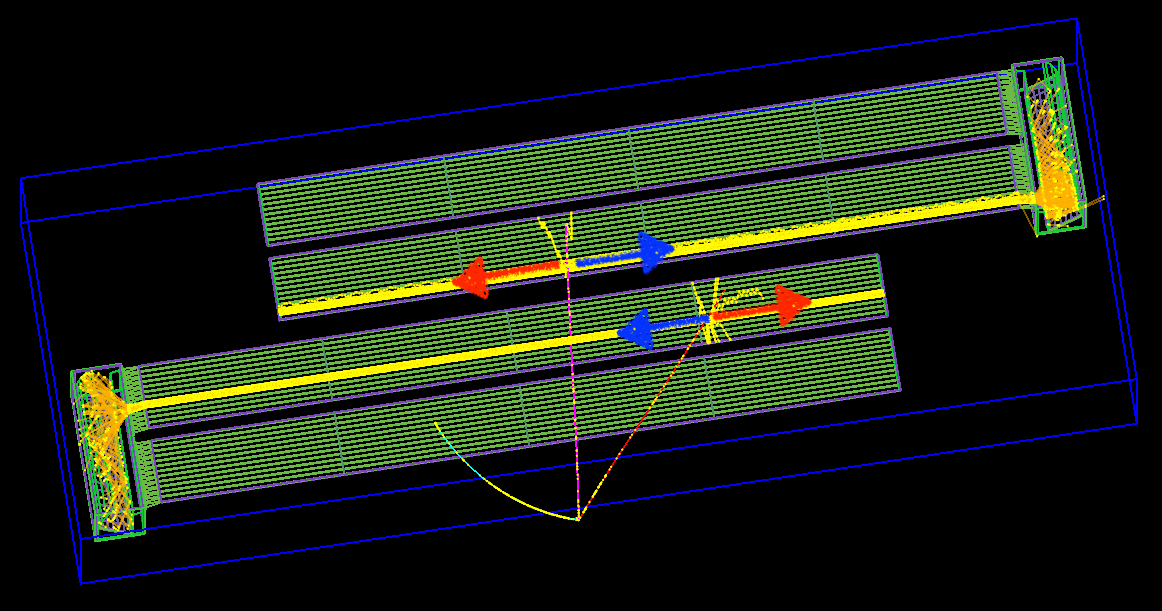
\includegraphics[width=0.75\textwidth]{pics/dir_ref.png}%eta2300decay.pdf}
\caption{\label{pic:eta2300}
An event showing the decay of $\eta(2300)$ into a kaon (red track) and a pion (magenta track). 
%A pion is shown in magenta, a kaon is shown in red. 
%A proton is shown in cyan. 
The pion and proton create Cherenkov photons (yellow tracks) inside two different DIRC radiators. The photons are transported to the optical boxes and imaged onto photodetection planes. The arrows indicate the direction of propagation for the photons going straight to the readout end of the bars (blue arrows), and photons which get reflected on the mirror at the bar end (red arrows). 
}
\end{figure}

Figure~\ref{pic:eta2300} shows a decay of $\eta(2300)$. The final state pion is shown in magenta and hits the upper bar box. The final state kaon is shown in red and hits the lower bar box. Both charged particles produce Cherenkov photons (their trajectories are shown in yellow), that propagate inside individual radiators towards the optical boxes, where they are detected. 
%An example of the single event hit pattern for a kaon and pion are shown in Fig.~\ref{pic:hitpat1} in the upper row. 

\begin{figure}[!h]
\centering
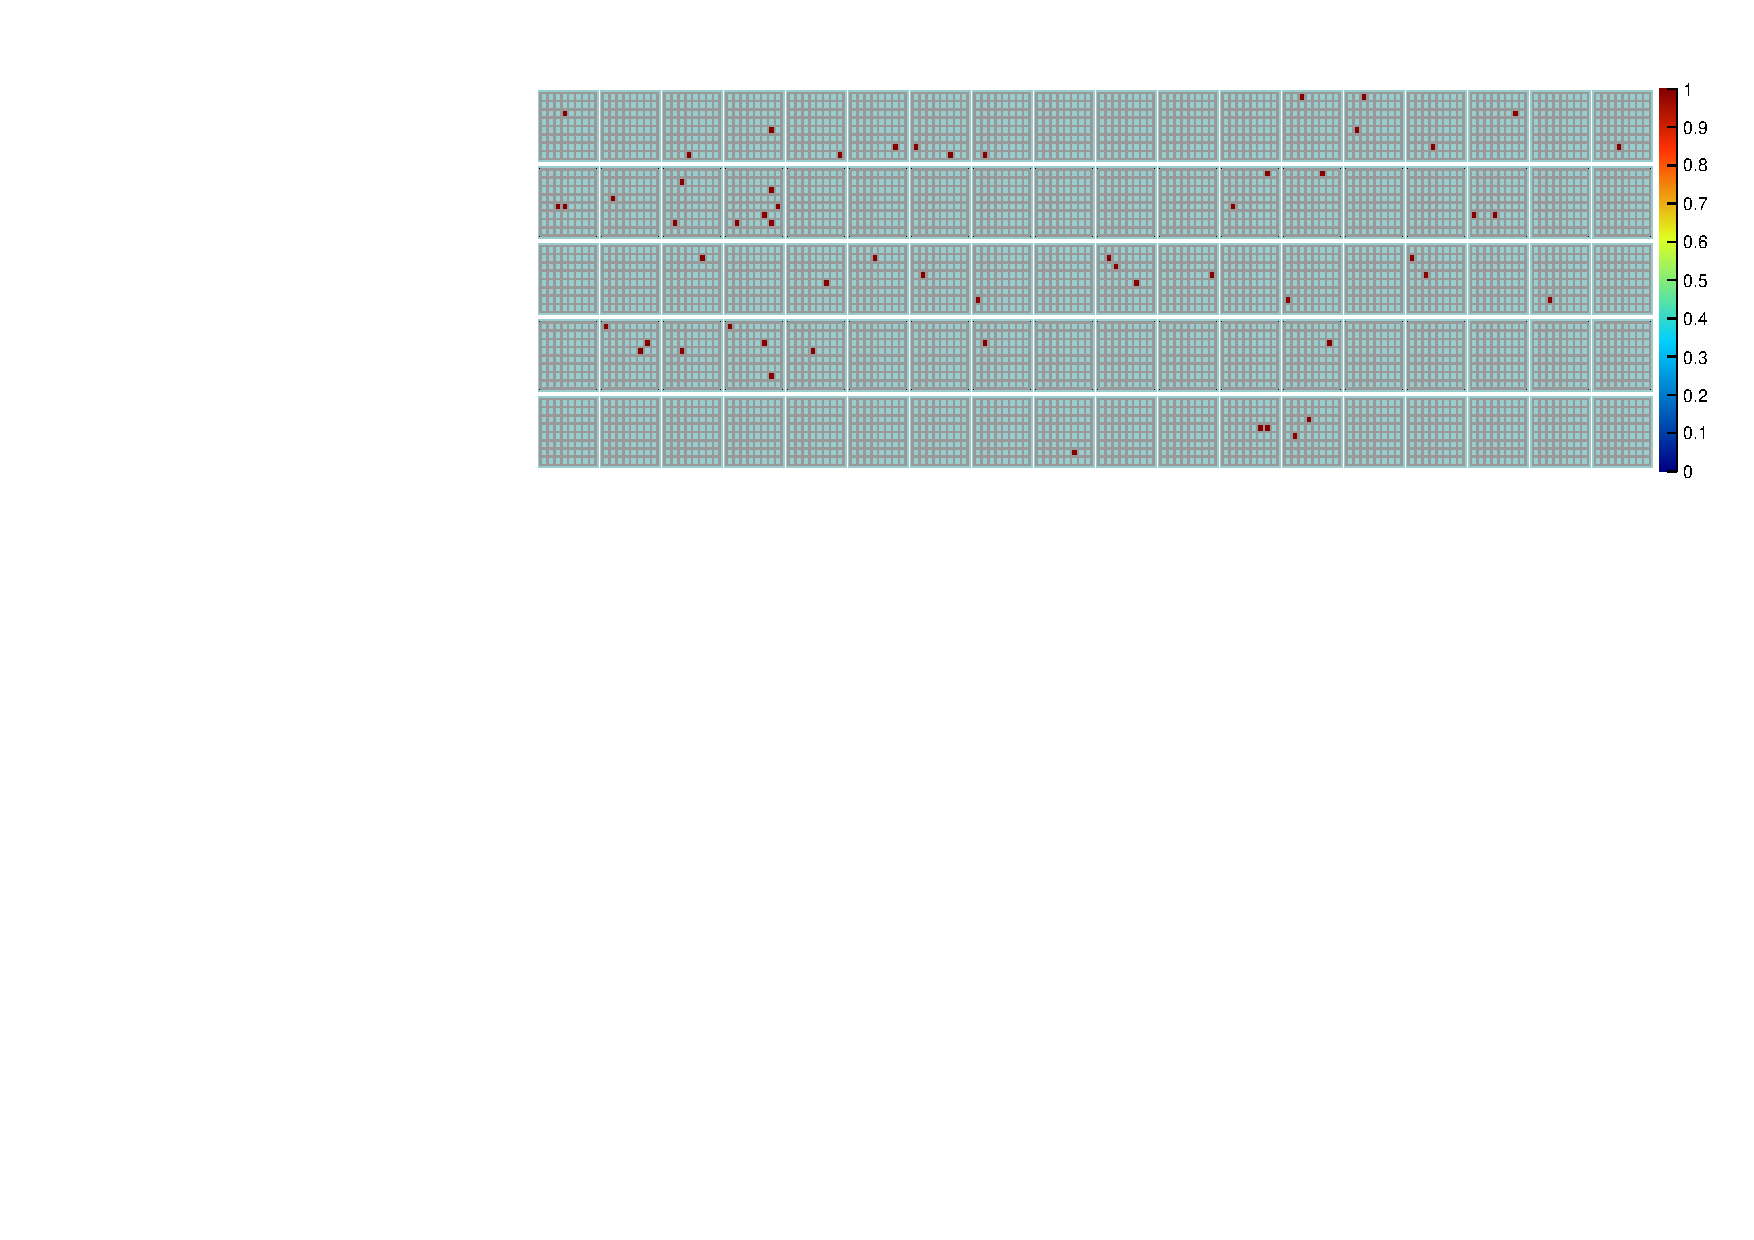
\includegraphics[angle=0,width=0.47\textwidth]{pics/kaon2GeVa.pdf} \hspace{0.5cm} 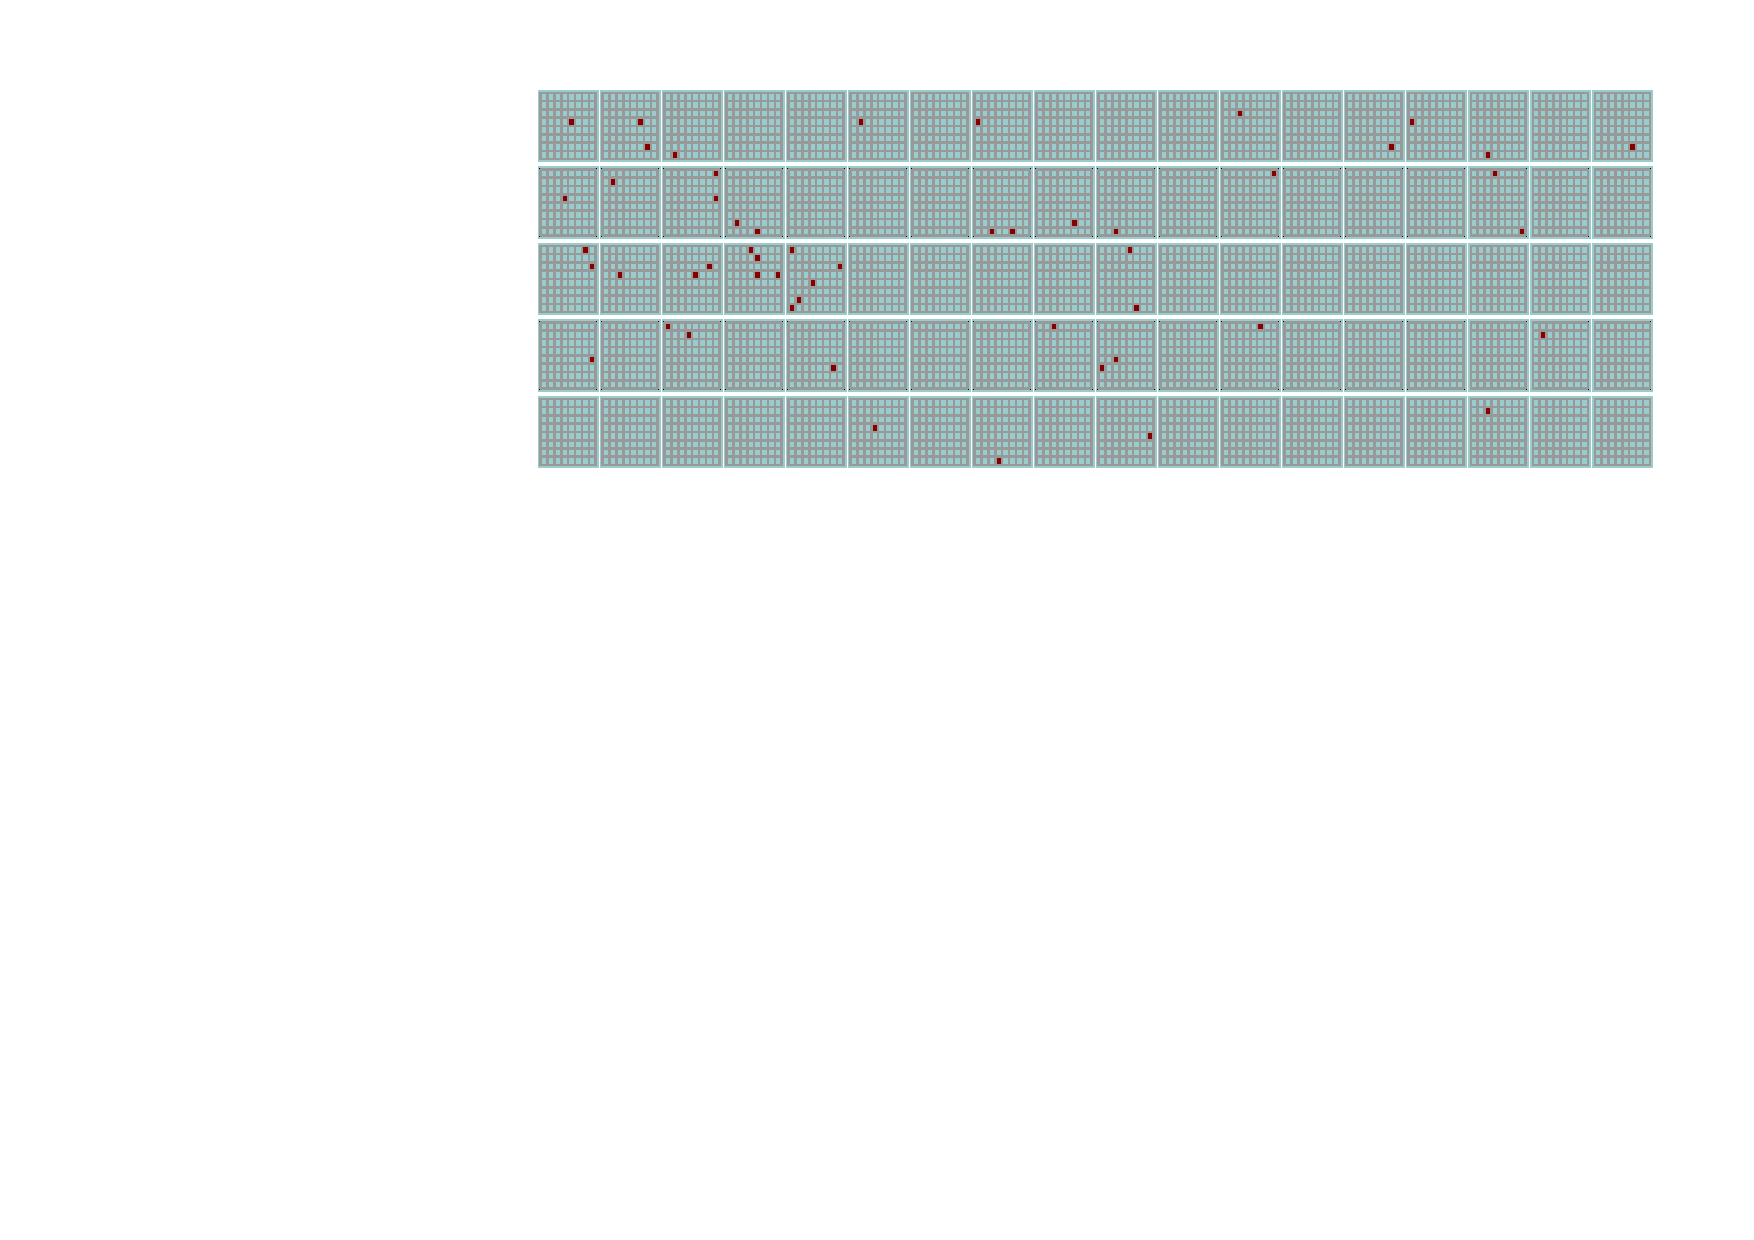
\includegraphics[angle=0,width=0.47\textwidth]{pics/pion2GeVa.pdf}\\
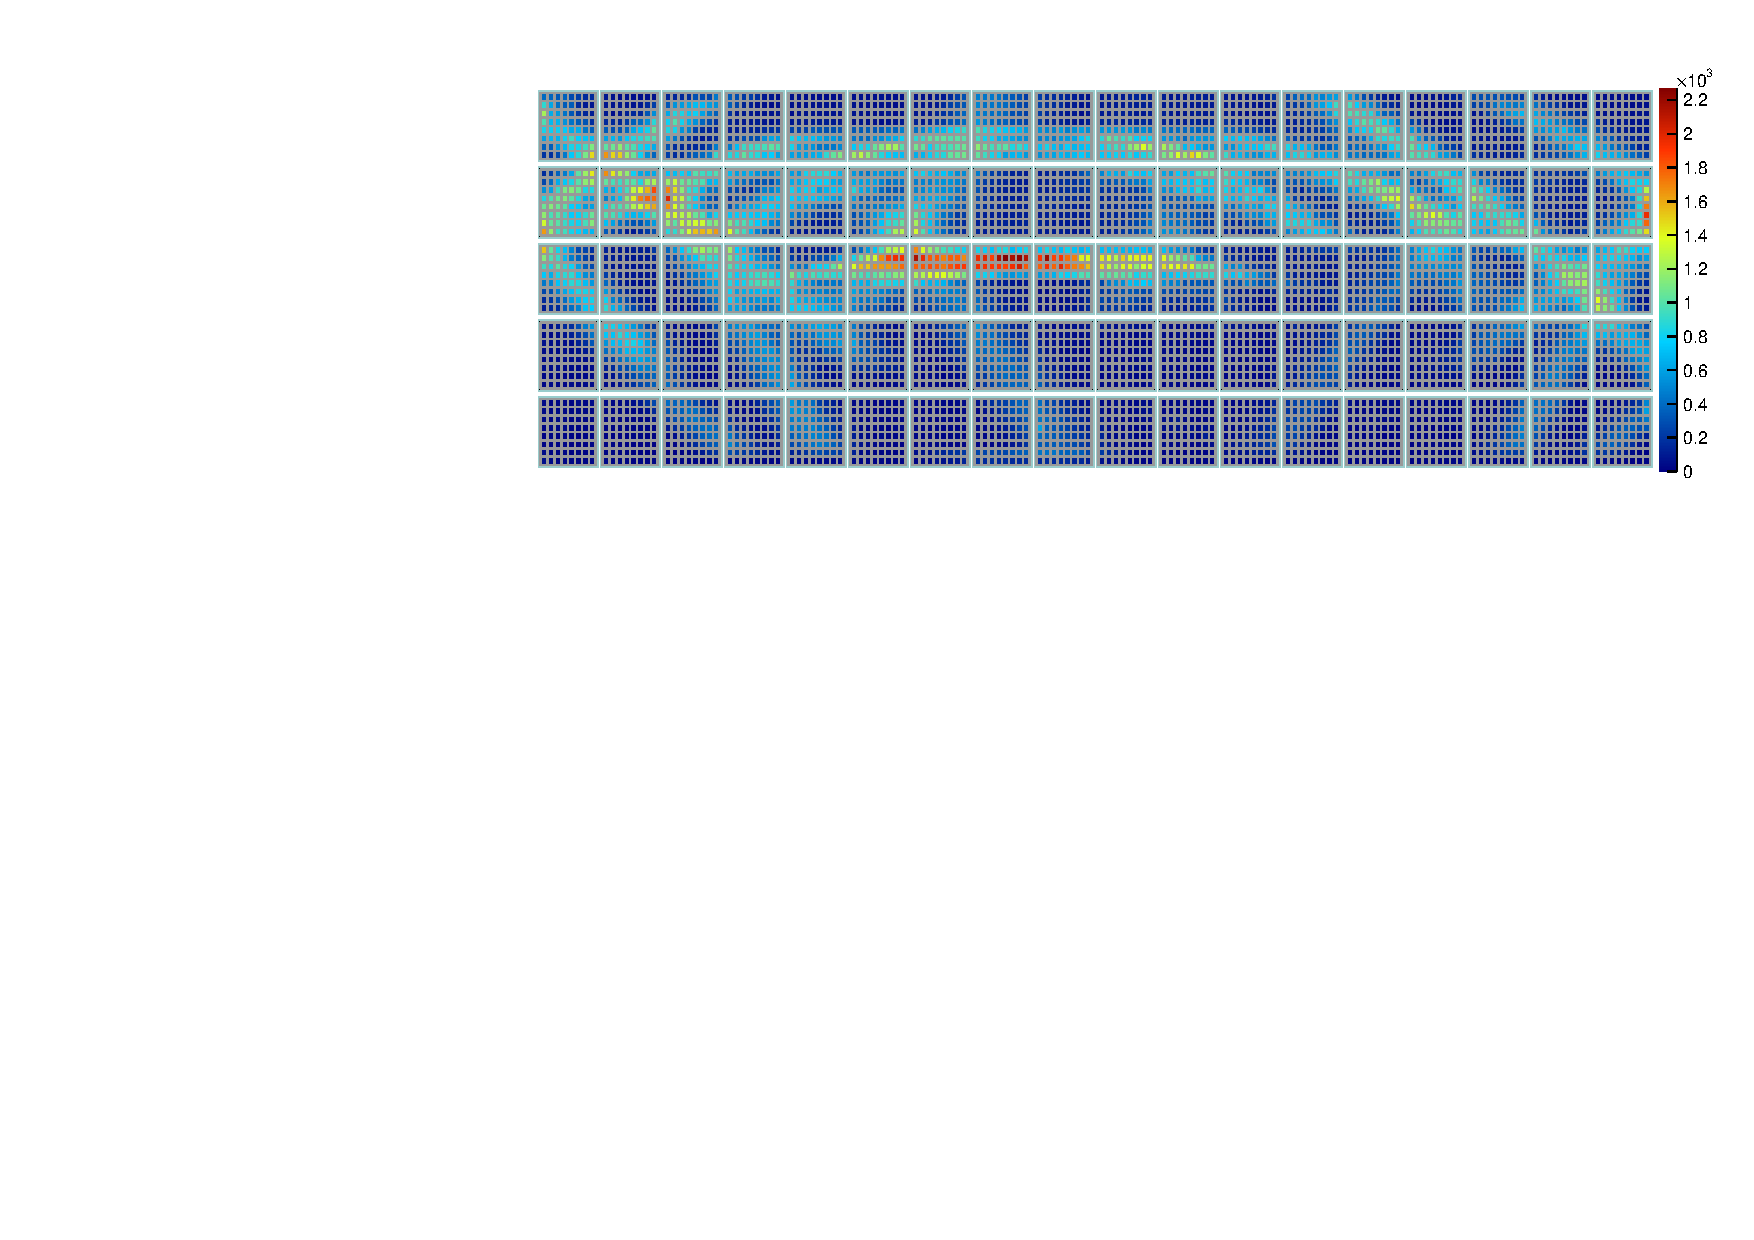
\includegraphics[angle=0,width=0.47\textwidth]{pics/kaons2GeV.pdf} \hspace{0.5cm} 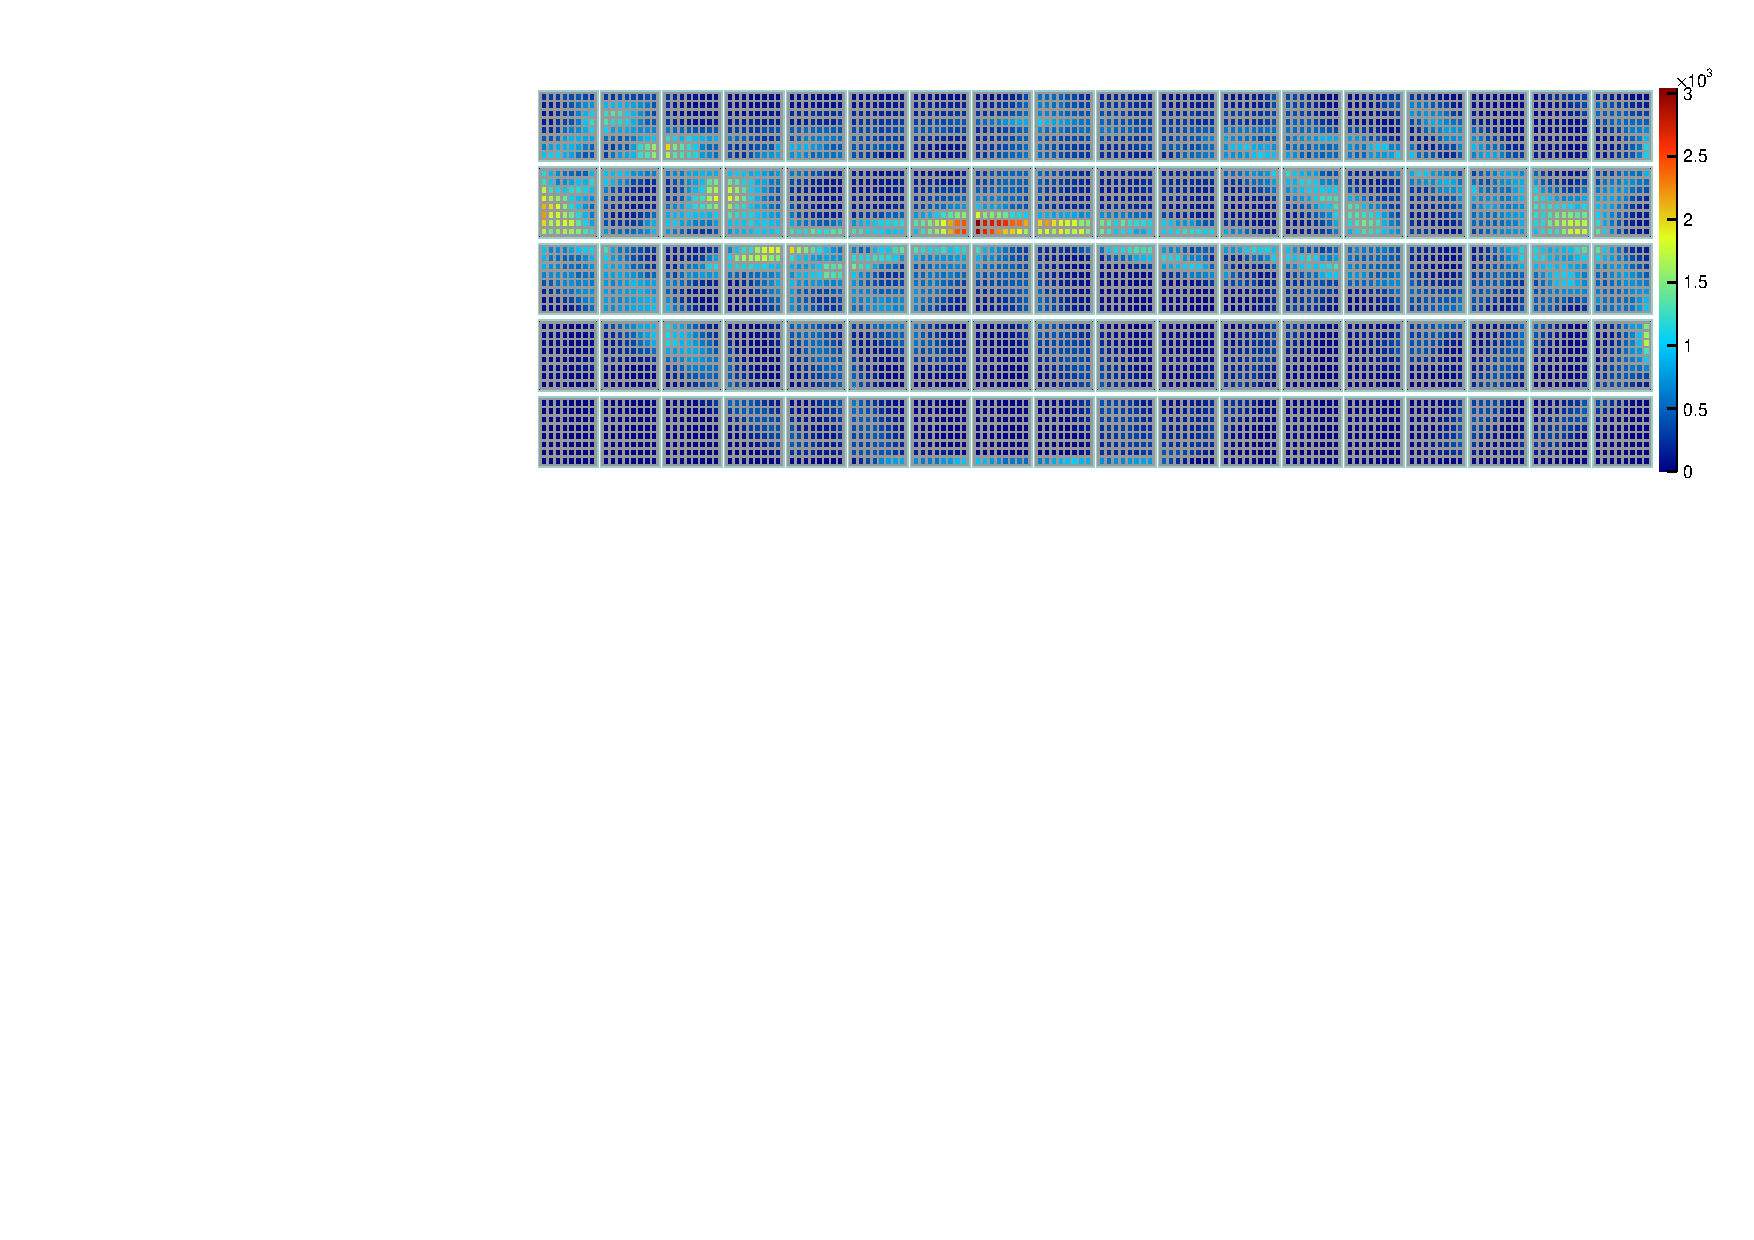
\includegraphics[angle=0,width=0.47\textwidth]{pics/pions2GeV.pdf}
\caption{\label{pic:hitpat1}
Typical \gluex DIRC hit patterns. The left column shows pions, and the right one -- kaons. 
Signals from single charged particles are shown in the upper row, and the cumulative patterns in the lower row.
One edge row of 18 PMTs is removed (should have been substituted with dummies. This idea then was transformed into distributing dummies according to the map shown in Fig.~\ref{pic:dummies}).
%Signals from single charged particles (upper row) look quite uncorrelated, and the cumulative patterns (bottom row) represent the complexity of the patterns. 
Samples of $40000$ single kaons and pions with momentum of 2 {\gev}/c and direction defined by $\theta = 1.2$\mydeg and $\phi = 90$\mydeg angles were used to create these plots.
}
\end{figure}

Typical \gluex DIRC hit patterns are shown in Fig.~\ref{pic:hitpat1}. DIRC does not try to reconstruct the shape of the hit pattern, but use different methods to compare hit patterns $(x,y,t)$\footnote{It is convenient to use a separate coordinate system on the photodetection plane. There $x$ axis goes along the long rows of PMTs containing $18$ sensors each, and $y$ axis goes along the short PMT rows of $6$ sensors each.} to expectations for different particle hypotheses ($e, \mu, \pi, K, p$).

%\begin{figure}[!h]
%\centering
%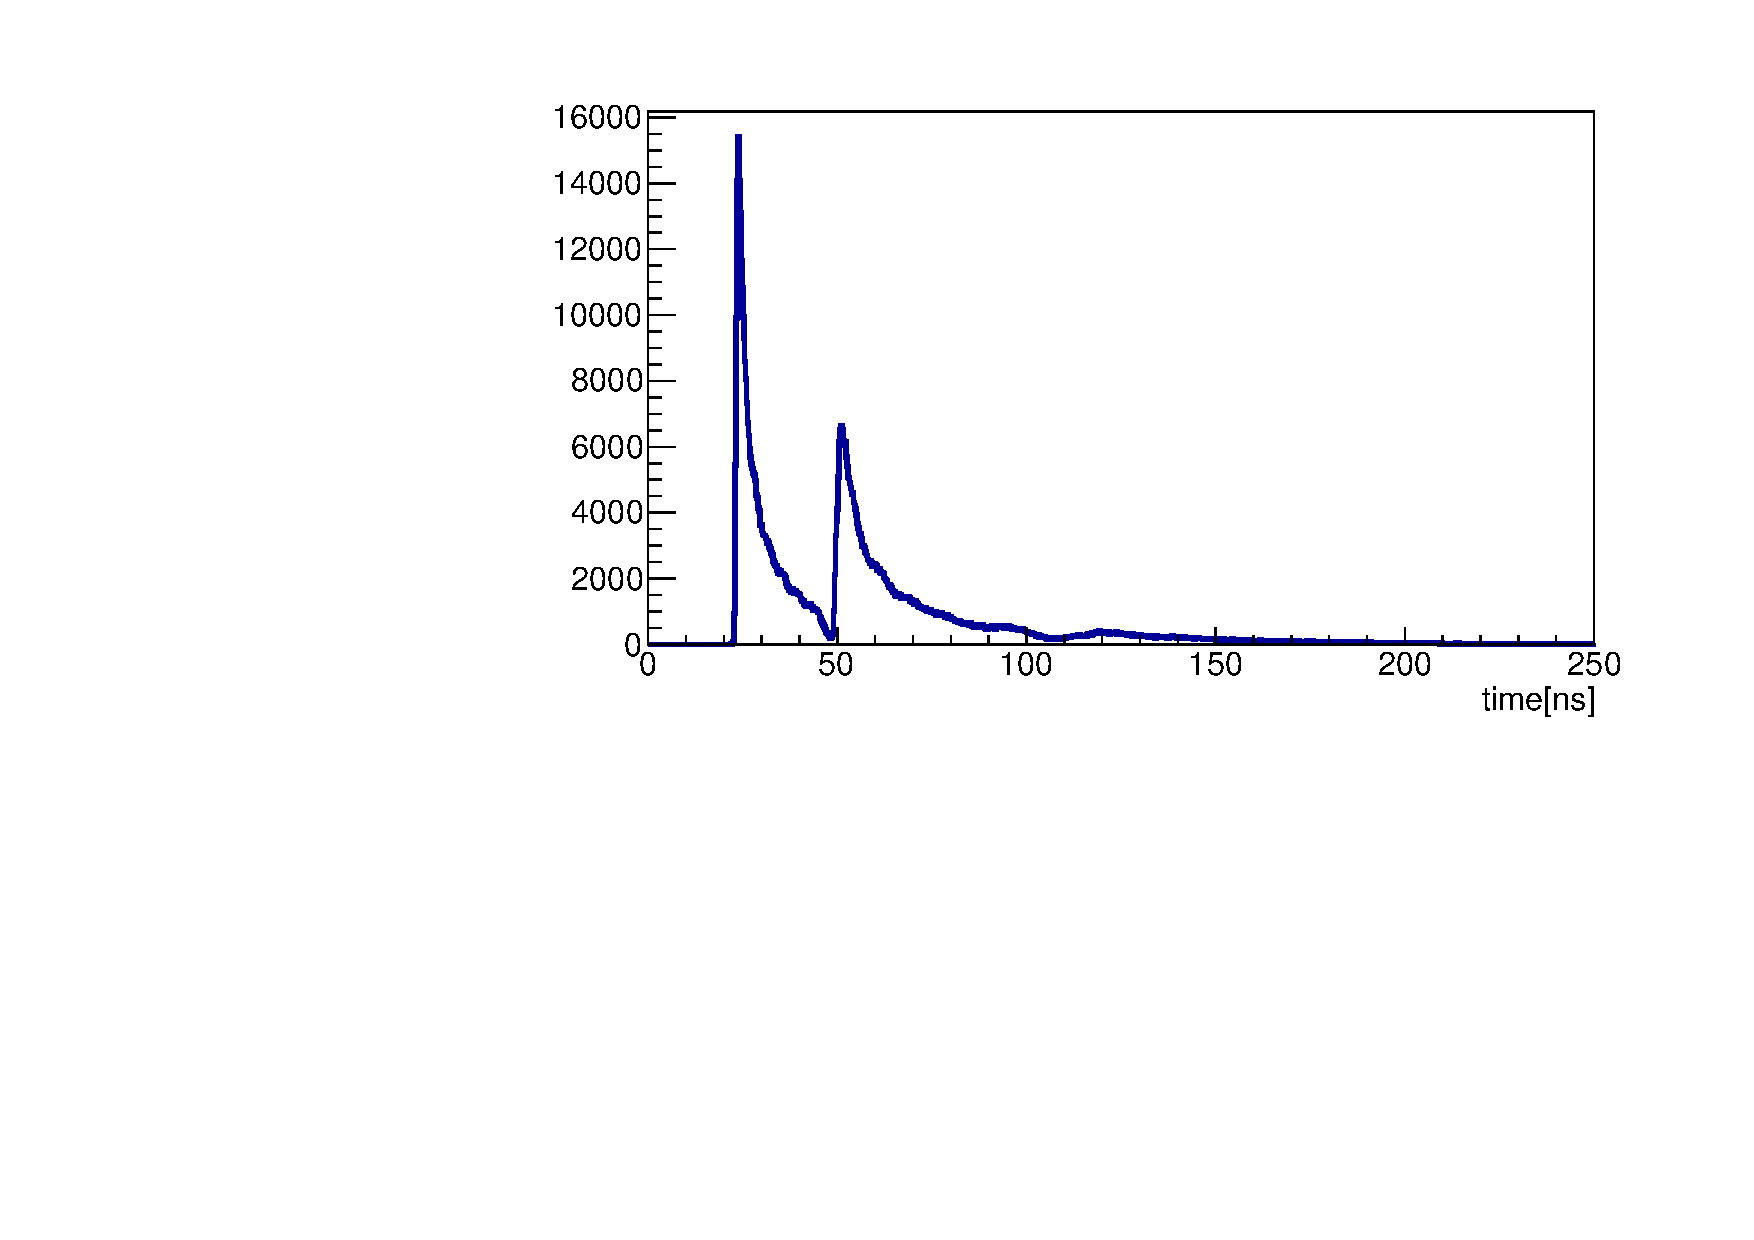
\includegraphics[angle=0,width=0.6\textwidth]{pics/Npho_th1_2_ph90.pdf}
%\caption{\label{pic:time}
%An example of the cumulative timing signal for charged kaons with momentum of 2 {\gev}/c and direction defined by $\theta = 1.2$\mydeg and $\phi = 90$\mydeg angles. The two peaks at $25$ ns and $55$ ns correspond to two groups of Cherenkov photons. The first group (left peak) contains direct photons, which were emitted towards the readout end of the bar unlike the second group (right peak), which first went to the mirror at the fuar end of the radiator, and then towards the optical box. The spread of the timing signal for one track is tens of nanoseconds. 
%The dip in the spectra around $48$ ns show photon loss due to the total internal reflection inside the radiator. 
%}
%\end{figure}

DIRC measures $(x,y,t)$ of each detected Cherenkov photon. In $(x,y)$ the cumulative hit patterns look like conic sections with additional reflections (see cumulative hit patterns for different charged particle configurations \url{http://web-docs.gsi.de/~rdzhigad/www/research/hit-pattern-vs-theta-phi}). In the coordinate space ($x ,y$) some parts overlap, but timing helps to separate them.
The exact way to use the timing information for the reconstruction will be discussed in the next sections.
%An example of the cumulative timing spectra for charged kaons with fixed momentum and direction is shown in Fig.~\ref{pic:time}. 

The number of detected photons is an important observable of the DIRC. A comparison between the measured and expected photon yield for different hypotheses at a given momentum help to separate between different particle types. Examples of the simulated number of detected photons for kaons and pions with different momenta are shown in Fig.~\ref{pic:npho}.

\begin{figure}[!h]
\centering
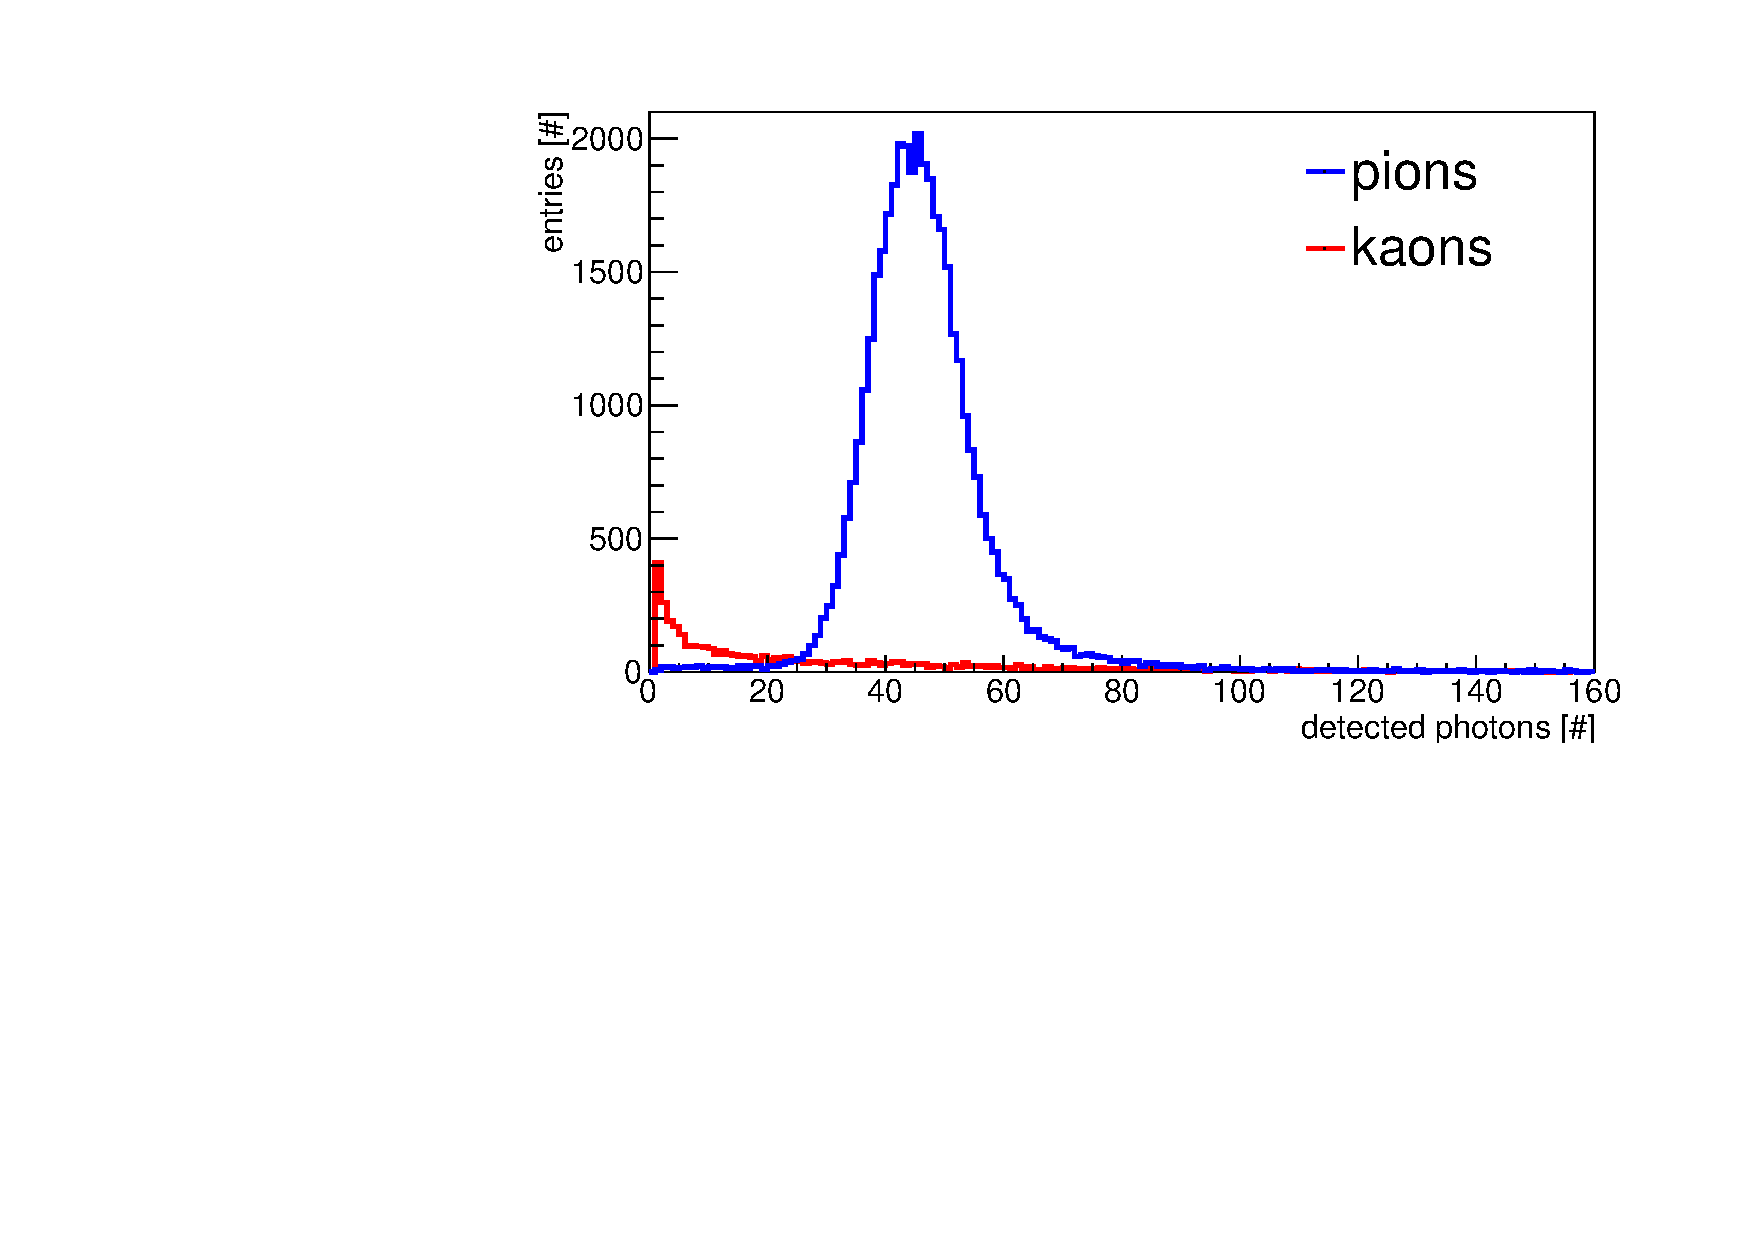
\includegraphics[width=0.43\textwidth]{pics/Npho0_5GeV.pdf} \put(-80.,50.){0.5 GeV/c} \hspace{0.5cm} 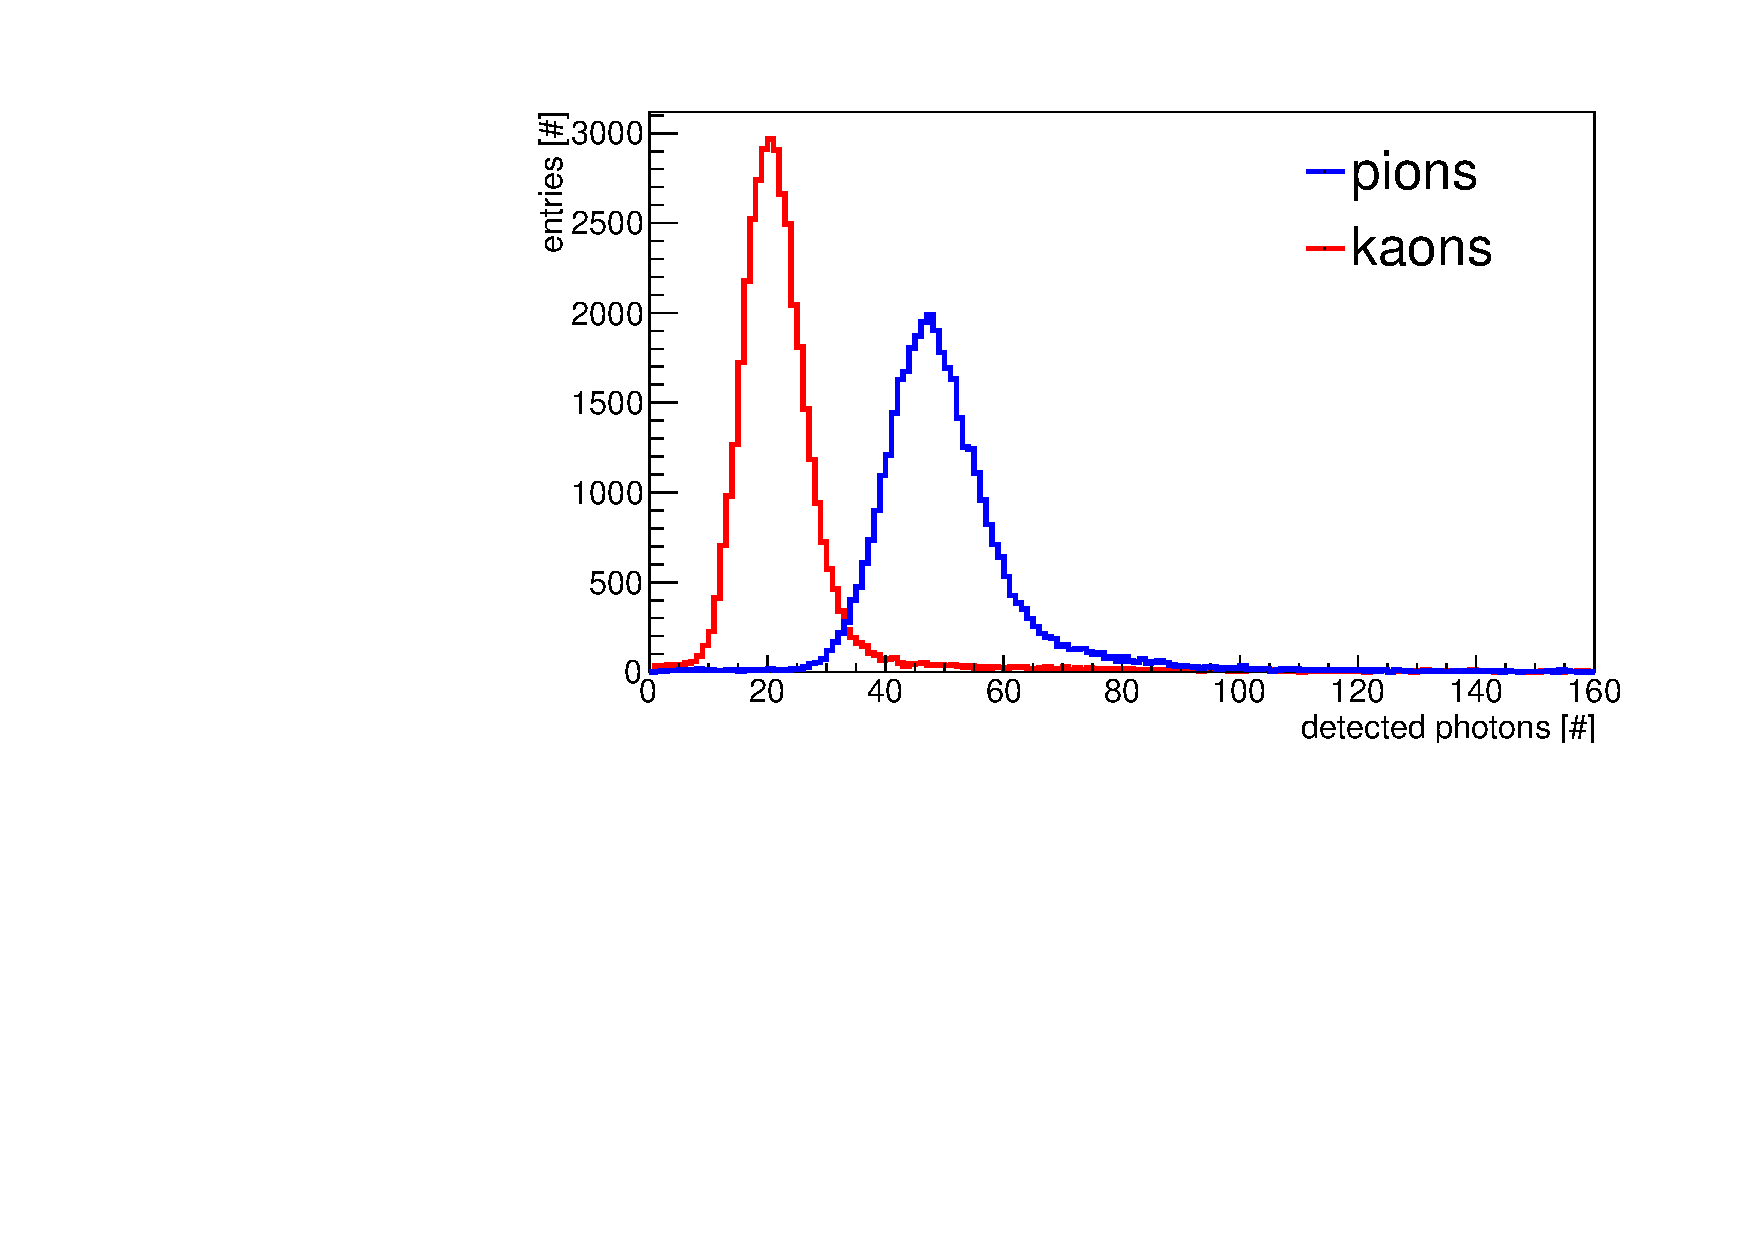
\includegraphics[width=0.43\textwidth]{pics/Npho0_8GeV.pdf} \put(-80.,50.){0.8 GeV/c}\\
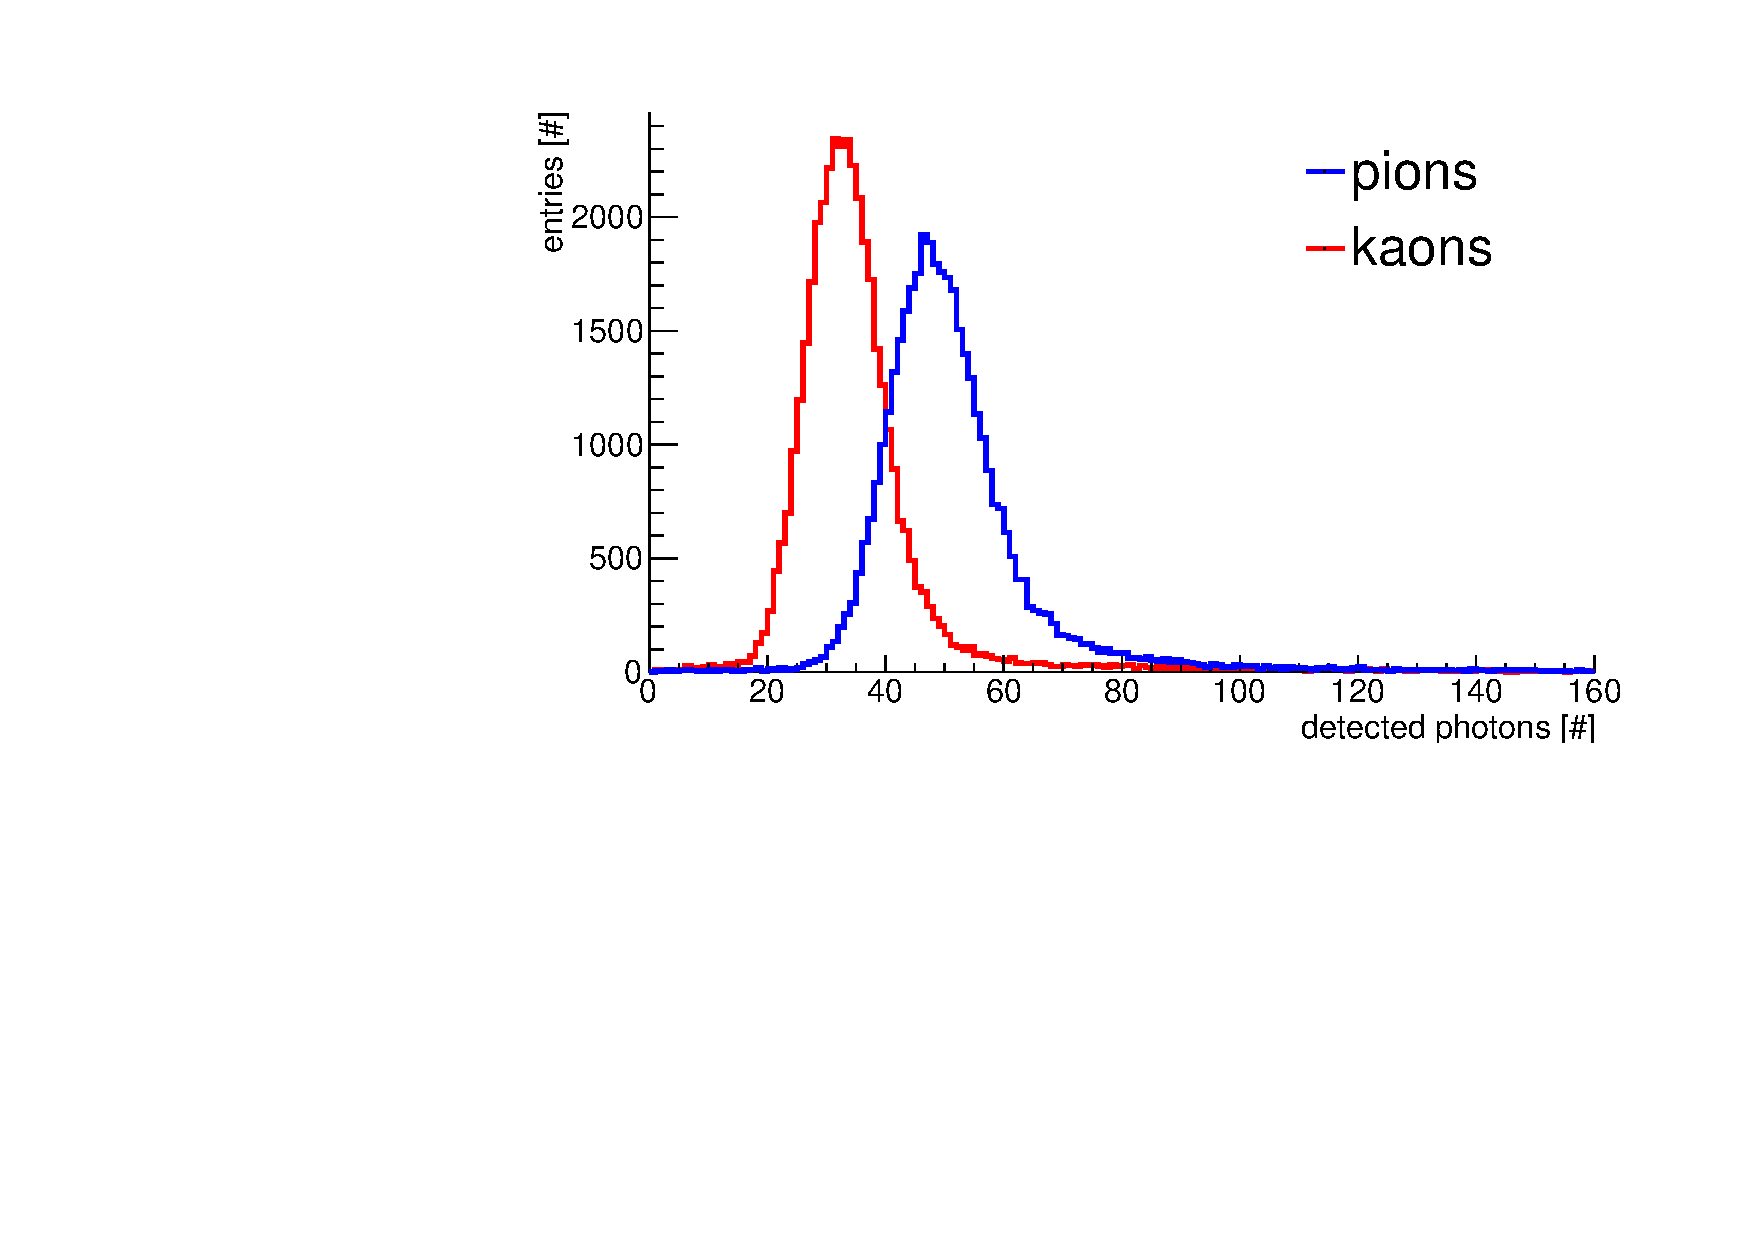
\includegraphics[width=0.43\textwidth]{pics/Npho1GeV.pdf} \put(-80.,50.){1 GeV/c} \hspace{0.5cm} 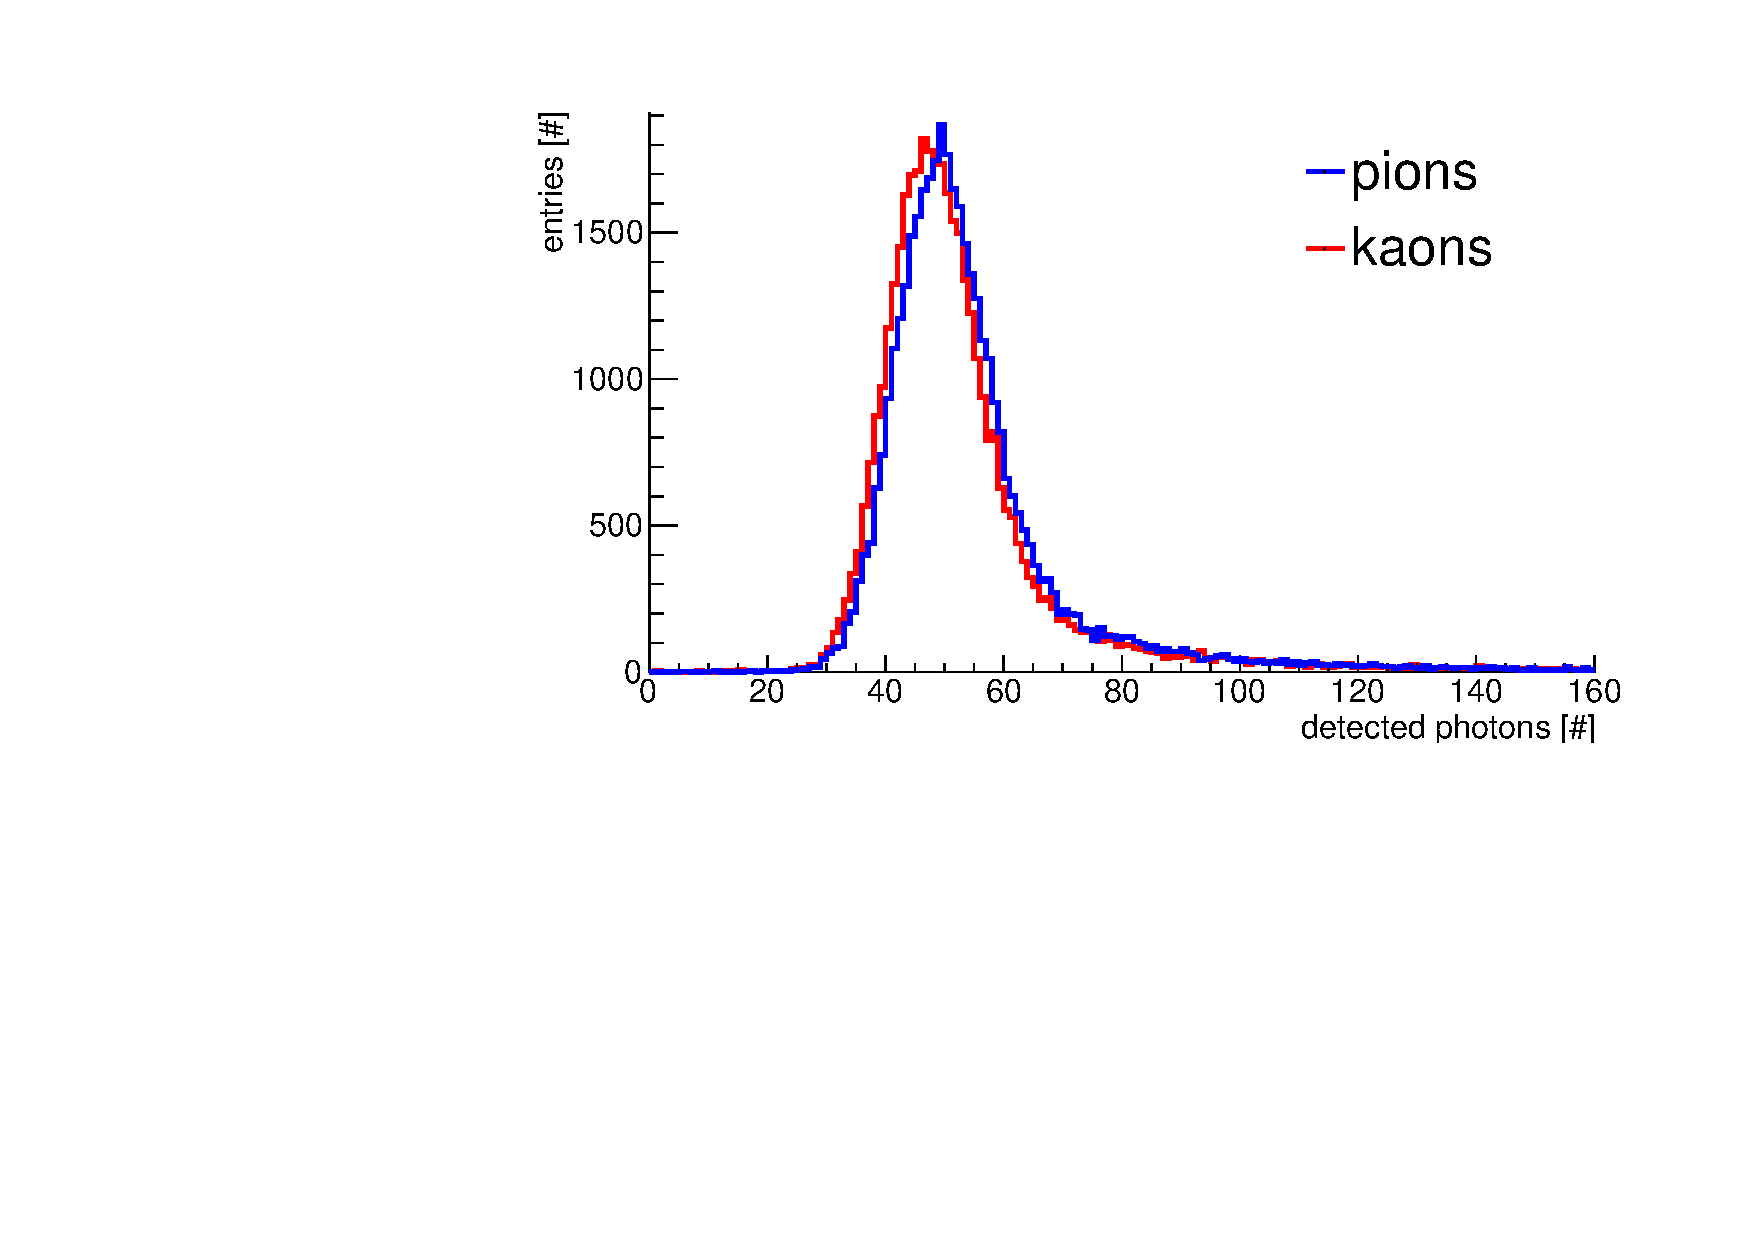
\includegraphics[width=0.43\textwidth]{pics/Npho3GeV.pdf} \put(-80.,50.){3 GeV/c}\\
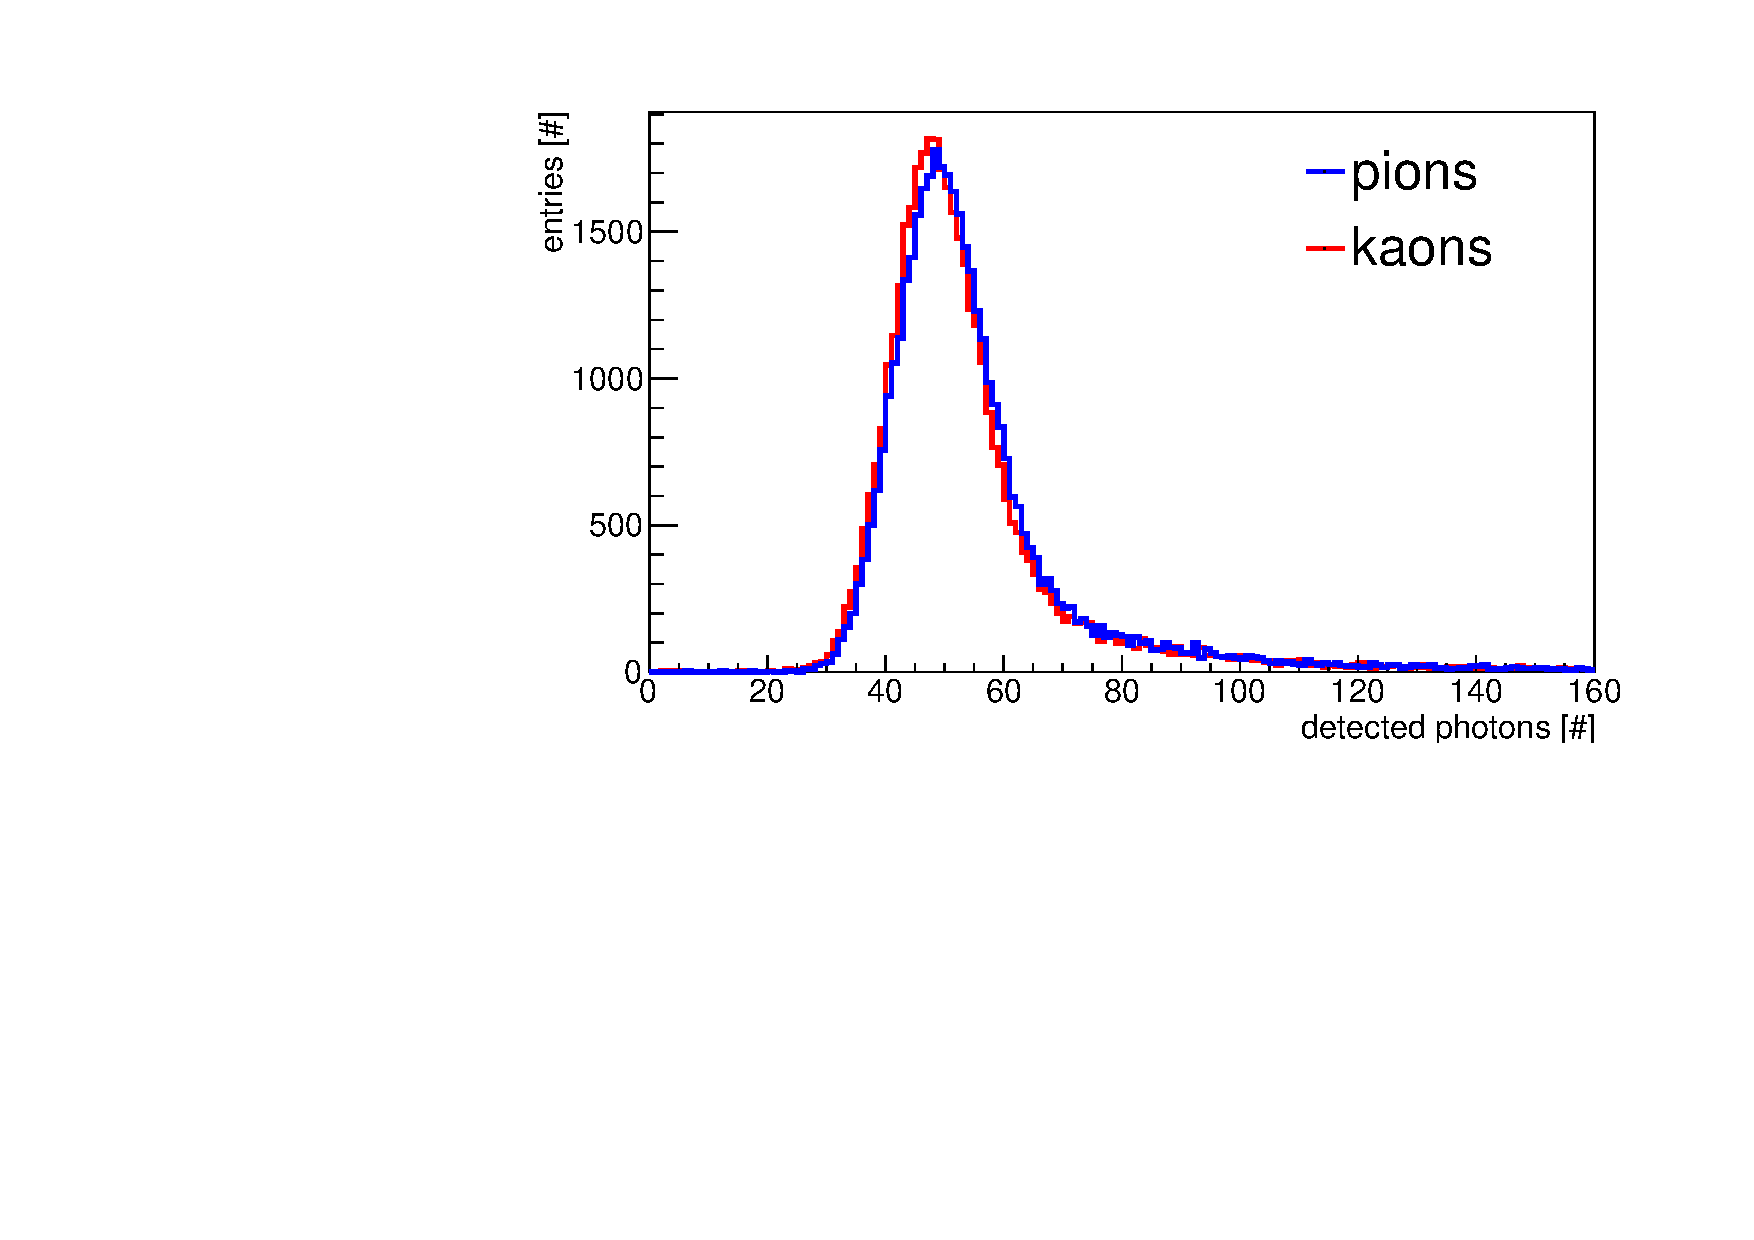
\includegraphics[width=0.43\textwidth]{pics/Npho4GeV.pdf} \put(-80.,50.){4 GeV/c} \hspace{0.5cm}
\caption{\label{pic:npho}
Simulated number of detected photons per track for kaons (red) and pions (blue) for particle direction defined by  $\theta = 4$\mydeg and $\phi = 90$\mydeg and different momenta.
}
\end{figure}

\begin{figure}[!h]
\centering
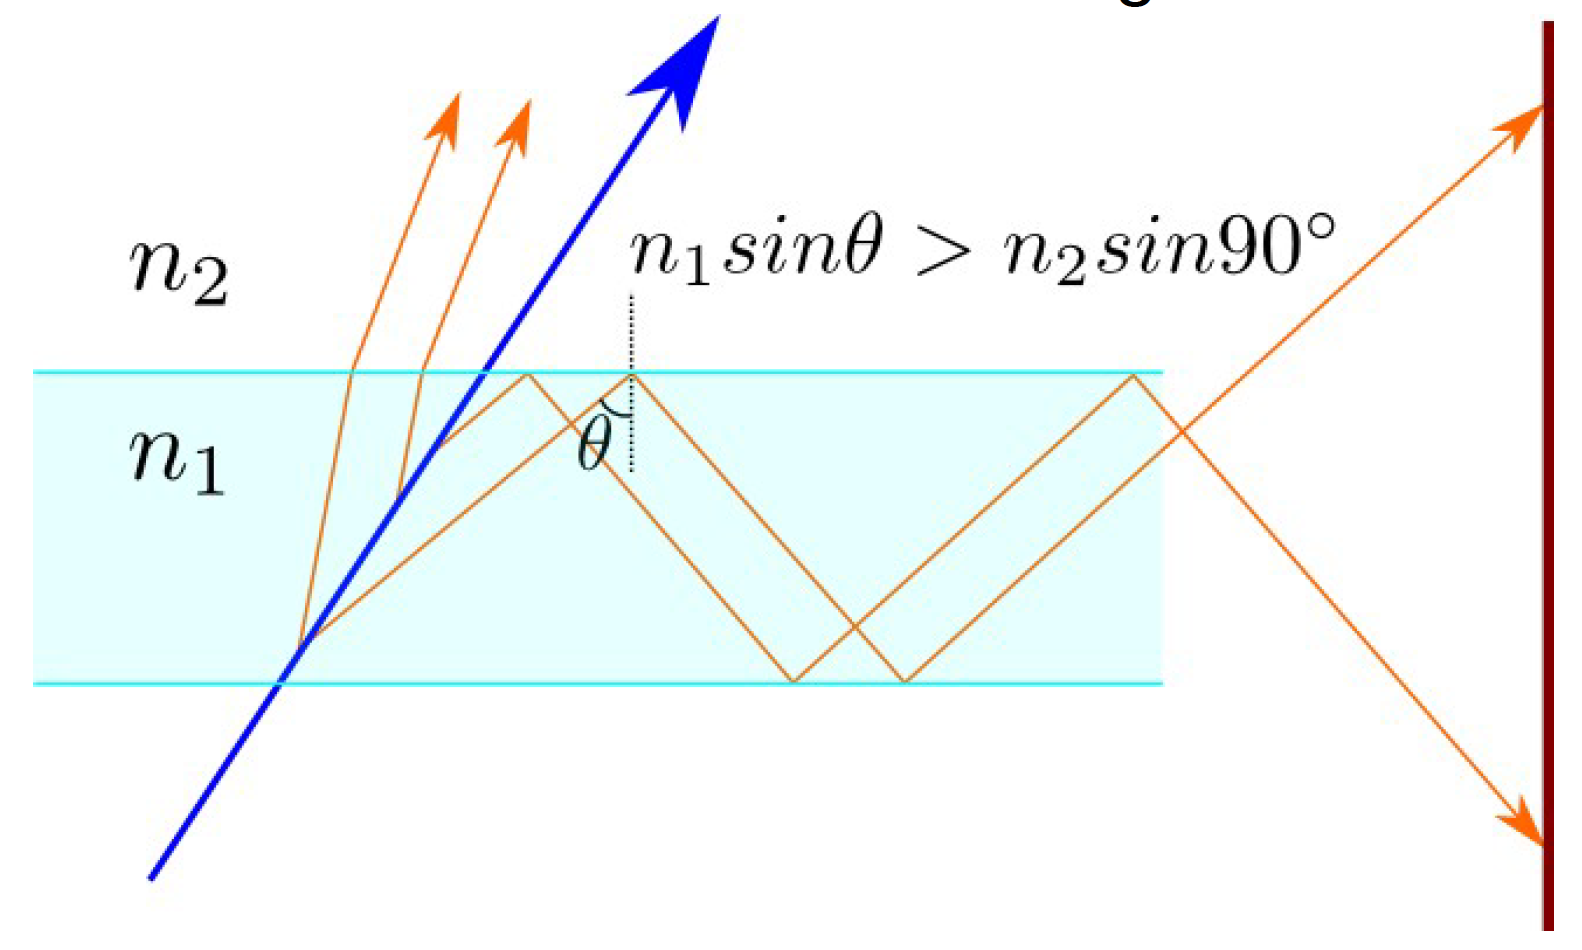
\includegraphics[width=0.5\textwidth]{pics/bas2.png}
\caption{\label{pic:bas2}
Illustration of the total internal reflection condition on the border between the fused silica ($n_{1}$) and air ($n_{2}$). Some Cherenkov photons do not satisfy the total internal reflection condition and escape the radiator. A fraction of the Cherenkov cone is internally reflected and thus can be transported to the photon detectors.
}
\end{figure}

DIRC has a specific timing signal with duration up to 100 ns. The formation of the signal is the following. When a charged particle crosses the radiator and produces Cherenkov photons on a cone, the total internal reflection condition defines which parts of the cone get trapped inside the radiator. Figure~\ref{pic:bas2} shows the case when the charged particle crosses the radiator at a rather shallow angle, so that only one side of the Cherenkov cone gets totally internally reflected. In case when the charged particle crosses the radiator almost perpendicularly, both sides of the Cherenkov cone satisfy the total internal reflection condition and, therefore, Cherenkov photons propagate towards both ends of the radiator. The ``direct'' photons propagate from the point of origin directly to the readout end of the bar (Fig.~\ref{pic:eta2300}, blue arrows), and ``reflected'' ones first go towards the bar end equipped with a mirror (Fig.~\ref{pic:eta2300}, red arrows). 

The DIRC timing signal might have one or two sharp time peaks, depending on the angle of the charged particle relative to the radiator sides. These time peaks correspond to direct and reflected photons. Examples of timing spectra for different radiators and several x positions of the charged particle along the DIRC radiator are shown in Fig.~\ref{pic:timedist}. Direct and reflected photons are shown in blue and red respectively.

\begin{figure}[!h]
\centering
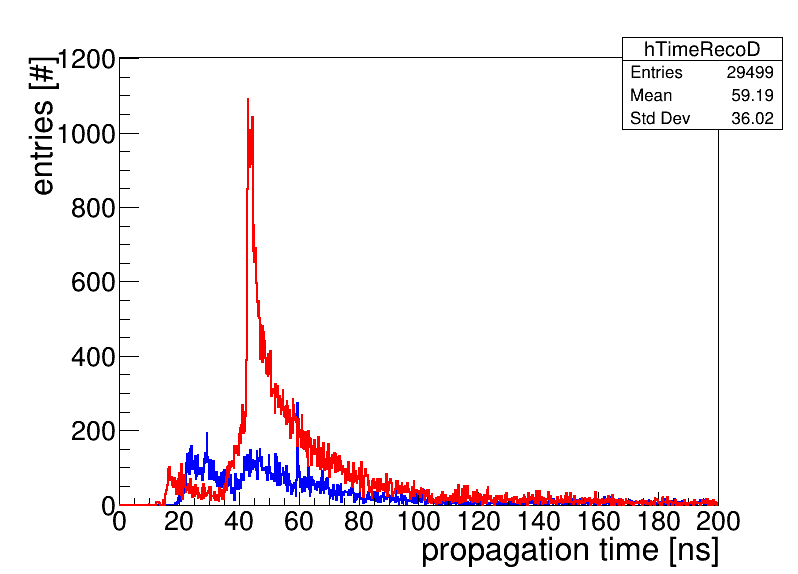
\includegraphics[width=0.45\textwidth]{pics/bar0_xm65.png} \put(-80.,90.){bar 0} \put(-80.,60.){x = -65 cm} \hspace{0.5cm} 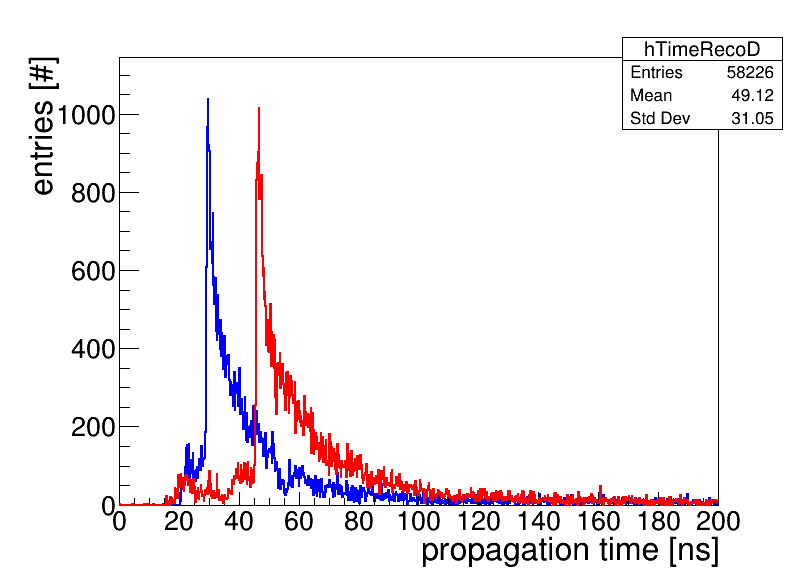
\includegraphics[width=0.45\textwidth]{pics/bar0_xm40.png} \put(-80.,90.){bar 0} \put(-80.,60.){x = -40 cm}\\
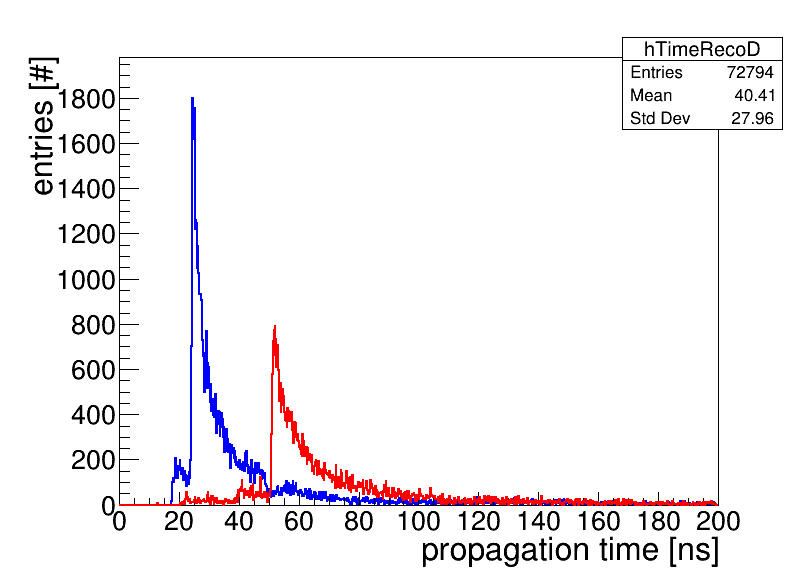
\includegraphics[width=0.45\textwidth]{pics/bar0_x0.png} \put(-80.,90.){bar 0} \put(-80.,60.){x = 0} \hspace{0.5cm} 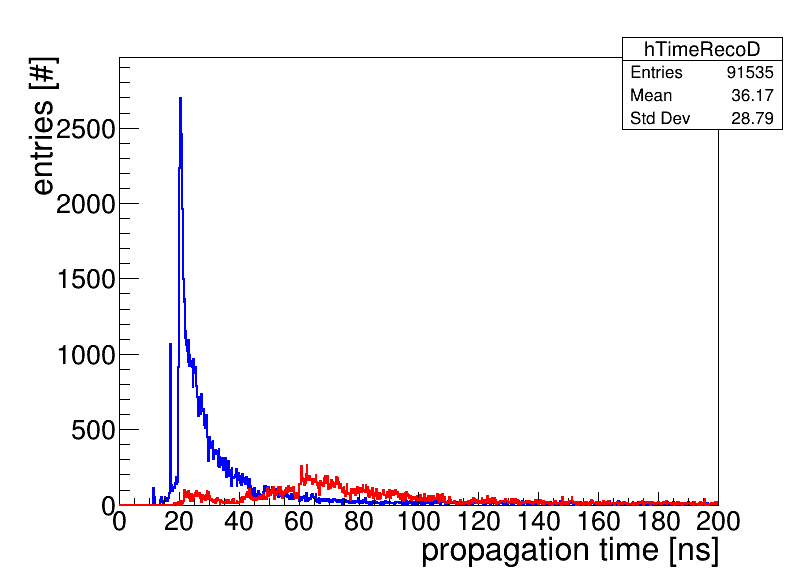
\includegraphics[width=0.45\textwidth]{pics/bar0_x45.png} \put(-80.,90.){bar 0} \put(-80.,60.){x = 45 cm}\\
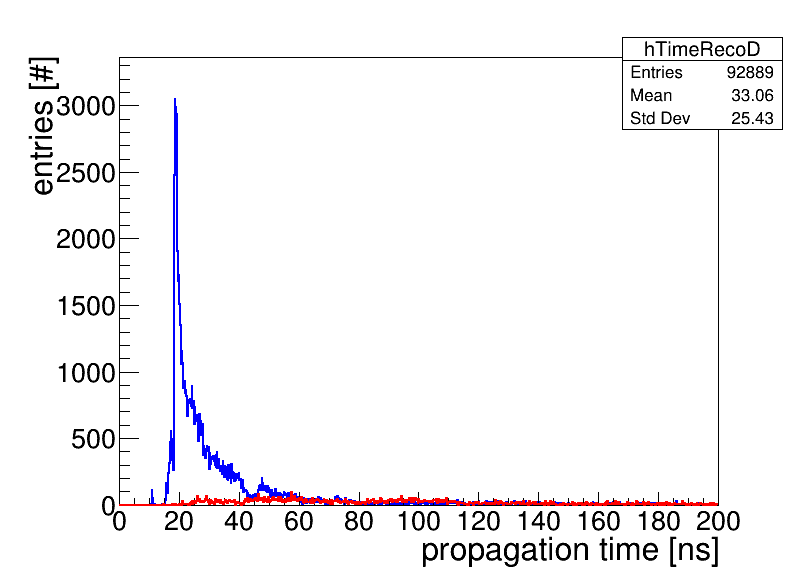
\includegraphics[width=0.45\textwidth]{pics/bar0_x65.png} \put(-80.,90.){bar 0} \put(-80.,60.){x = 65 cm} \hspace{0.5cm} 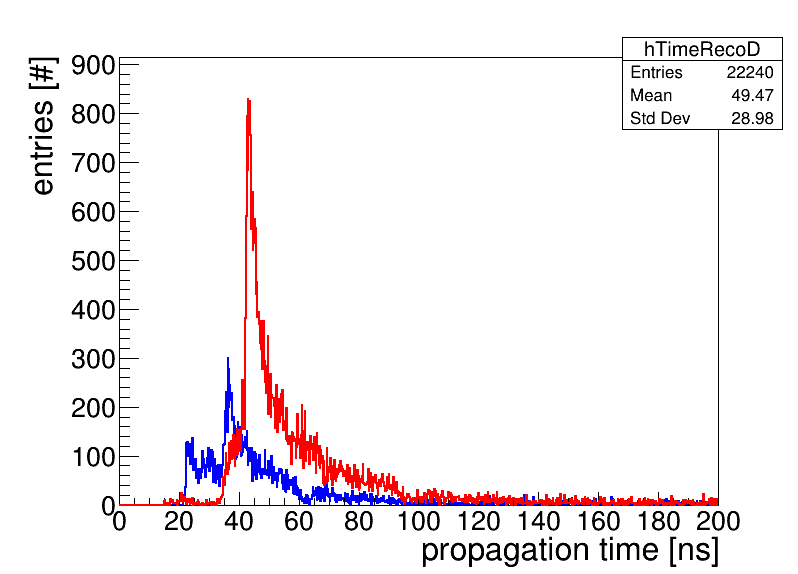
\includegraphics[width=0.45\textwidth]{pics/bar11_xm65.png} \put(-80.,90.){bar 11} \put(-80.,60.){x = -65 cm}
\caption{\label{pic:timedist}
Timing spectra for 500 single track events of kaons with momentum of 4 GeV/$c$ originating from the interaction point (0, 0, 65) cm and hitting radiators 0 and 11 at a given x position. The blue spectrum corresponds to the direct photons (see text for details), and the red spectrum -- for reflected photons. Irregular peaks like for bar 0, x = 45 cm at 17 ns correspond to signals from secondary particles.
}
\end{figure}